\documentclass[10pt,a4paper]{article}
\usepackage[T1]{fontenc}
\usepackage[polish]{babel}
\usepackage[utf8]{inputenc}
\usepackage{lmodern}
\usepackage{listings}
\selectlanguage{polish}
\usepackage[]{hyperref}
\usepackage{pdfpages}
\usepackage{float}
\newcommand\tab[1][0.5cm]{\hspace*{#1}}
\lstset{
  language=bash,
  basicstyle=\ttfamily,
  showstringspaces=false
}


\begin{document}


\title{Porównanie wizualizacji PCA i LDA}
\author{Bazyli Reps, Łukasz Knigawka}
\maketitle
\tableofcontents

\newpage

\section{Opis problemu}
Celem niniejszej pracy jest porównianie kompresji wymiarów danych za pomocą metod PCA oraz LDA. 
\\
Zamierzamy przedstawić przede wszystkim analizę redukcji wymiarowości dla obu metod, a następnie porównać je pod względem czasu wykonania redukcji a także uzyskanego stopnia kompresji. 
\\
Skrypty potrzebne do wykonania analiz napisane zostały w języku R.

\section{Opis danych}
Analizy przeprowadzone zostały na danych pobranych ze strony UCI Machine Learning Repository:
\url{http://archive.ics.uci.edu/ml/datasets/SPECTF+Heart}
\\
Przedstawiają one badania wyniki badań serca dla poszczególnych ROI (Region Of Interest) w zależności od stanu badanej osoby (w spoczynku lub podczs wysiłku).
\\
Dane zawierają 44 kolumny zawierające dane dla 22 ROI w obu stanach oraz jedną kolumnę opisującą która przyjmuje dwie wartości: 'normal' oraz 'abnormal'. Zestaw zawiera 265 rekordów.

\newpage
\section{Analiza PCA}
Dane zostały zredukowane do dwóch wymiarów. Na początku zostały wyznaczone wartości własne. 
\begin{figure}[H]
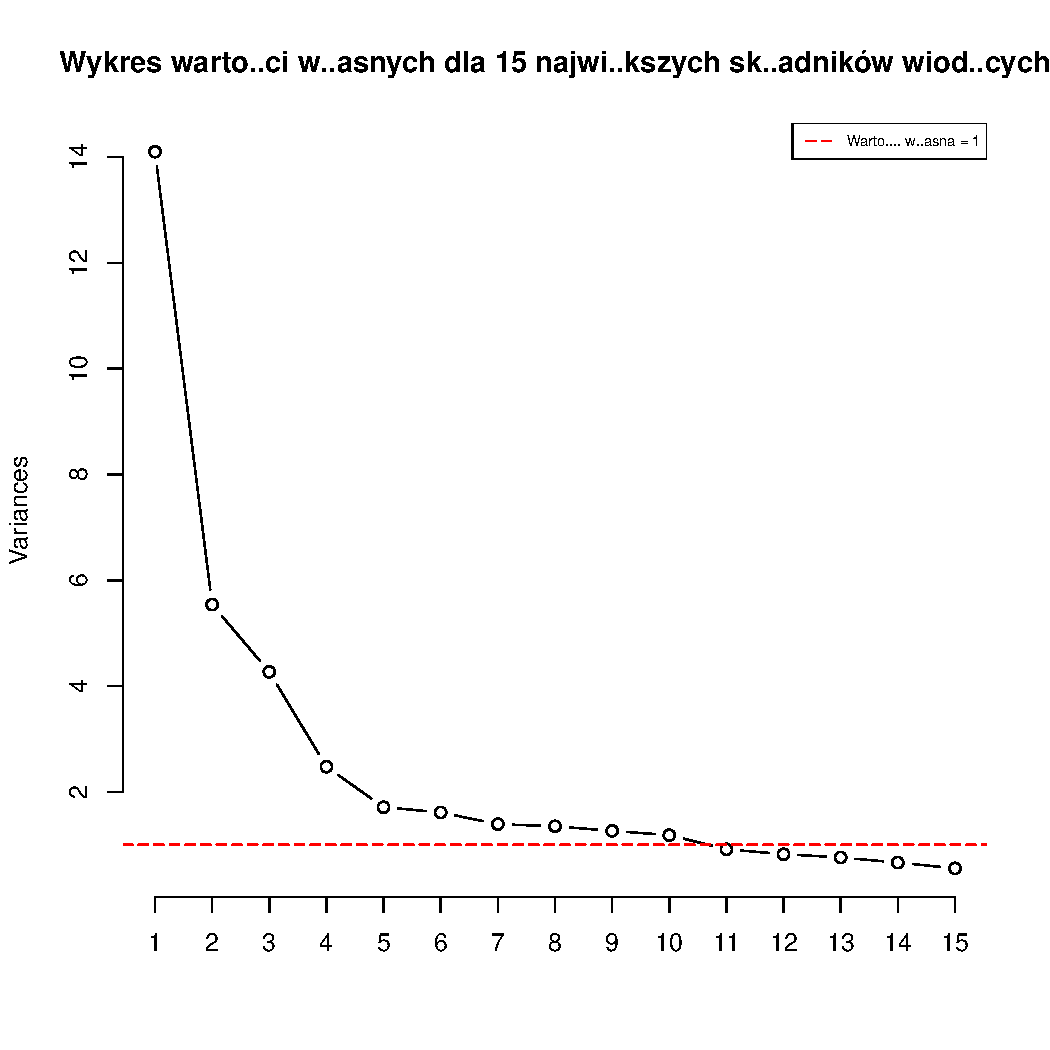
\includegraphics[scale=0.5]{wartosci_wlasne.pdf}
\caption{Istnieje dziesięć wartości własnych większych od 1. Pozostałe można swobodnie usunąć.}
\end{figure}

Następnie zbadana została wariancja wyjaśniona w zależności od ilości wziętych składników wiodących.
\begin{figure}[H]
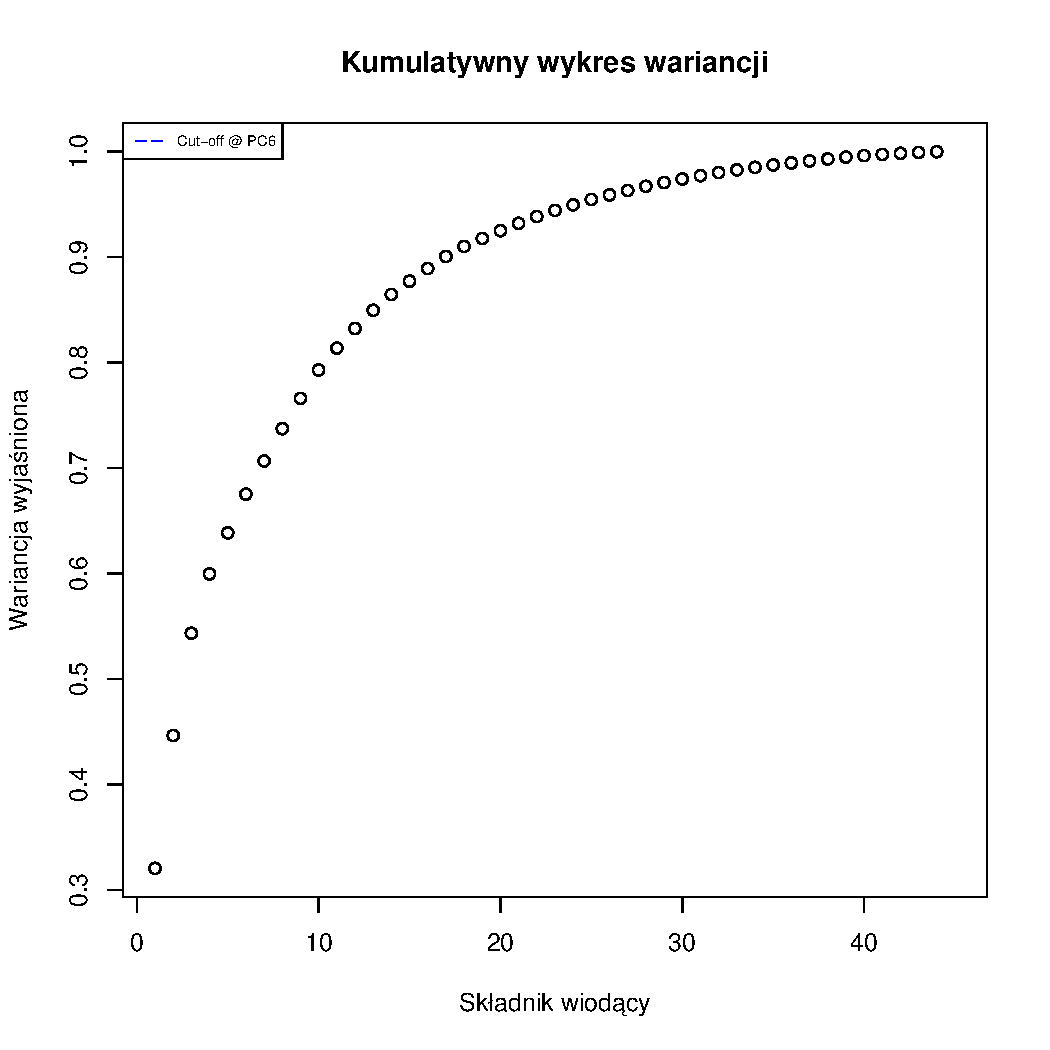
\includegraphics[scale=0.5]{wariancja_kum.pdf}
\caption{Największe dwa składniki wiodące wyjaśniają około 45\% wariancji danych}
\end{figure}

W dalszej kolejności zwizualizowane zostały dane po redukcji do dwóch wymiarów. Na wykresie zaznaczone zostały klasy obiektów.

\begin{figure}[H]
\includegraphics[scale=0.5]{klasy.pdf}
\caption{Wyraźnie widoczne jest zgrupowanie rekordów z diagnozowanych jako 'abnormal'. Niestety charakter danych, a co za tym idzie mniejsza od 60\% wyjaśniona wariancja powodują, że pomimo redukcji obie klasy nie są wyraźnie od siebie odseparowane.}
\end{figure}

\newpage
\section{Analiza LDA}
Dyskryminację liniową można wykorzystać w zadaniu redukcji wymiarowości, przy jej pomocy można zredukować liczbę wymiarów do N-1, gdzie N to liczba klas. LDA można także użyć jako klasyfikatora.
\\Aby przeprowadzić dyskryminację liniową dane zostały podzielone na zbiór treningowy oraz testowy (w klasycznych proporcjach odpowiednio 75\% oraz 25\% obserwacji). Dane zostały przeskalowane. Po nauczeniu klasyfikatora zbadaliśmy funkcje dyskryminacji dla poszczególnych klas.

\begin{figure}[H]
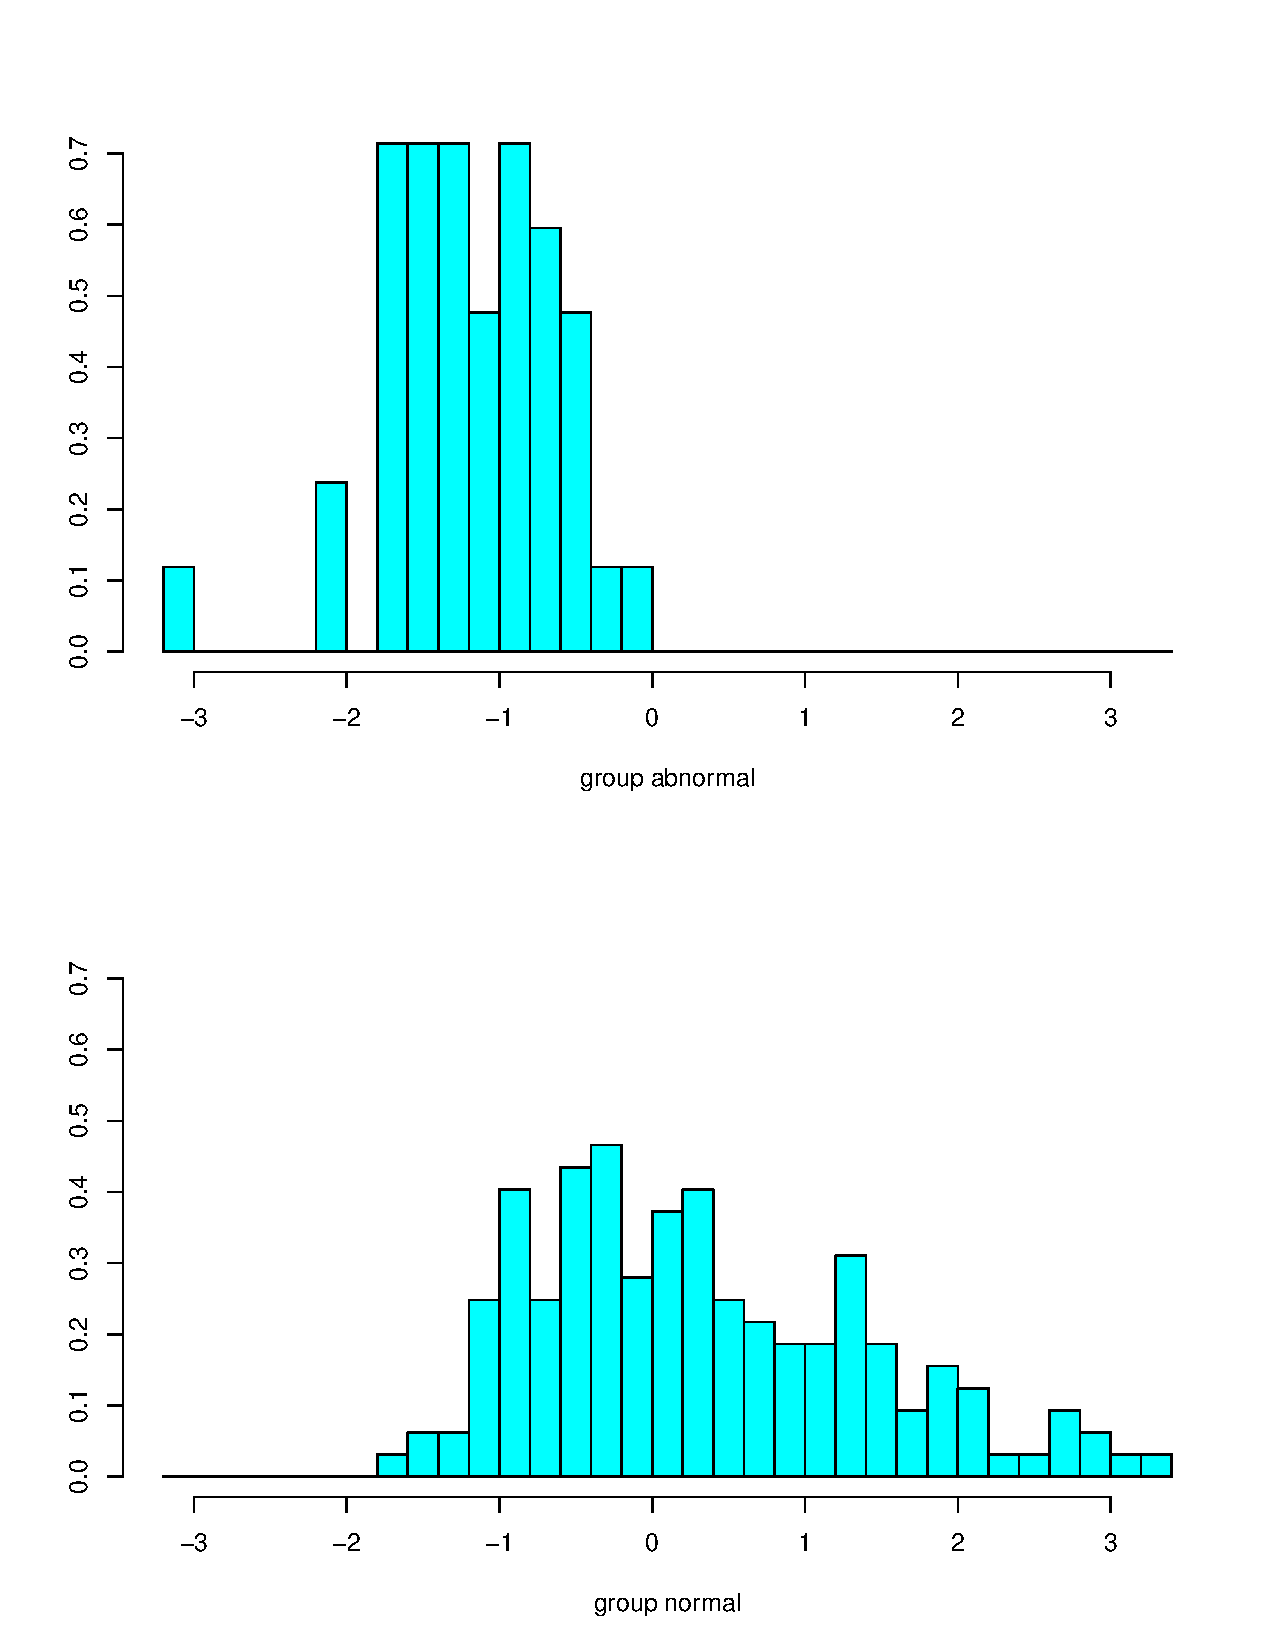
\includegraphics[scale=0.5]{ldahist.pdf}
\caption{Histogramy funkcji dyskryminacji dla poszczególnych klas}
\end{figure}

\begin{figure}[H]
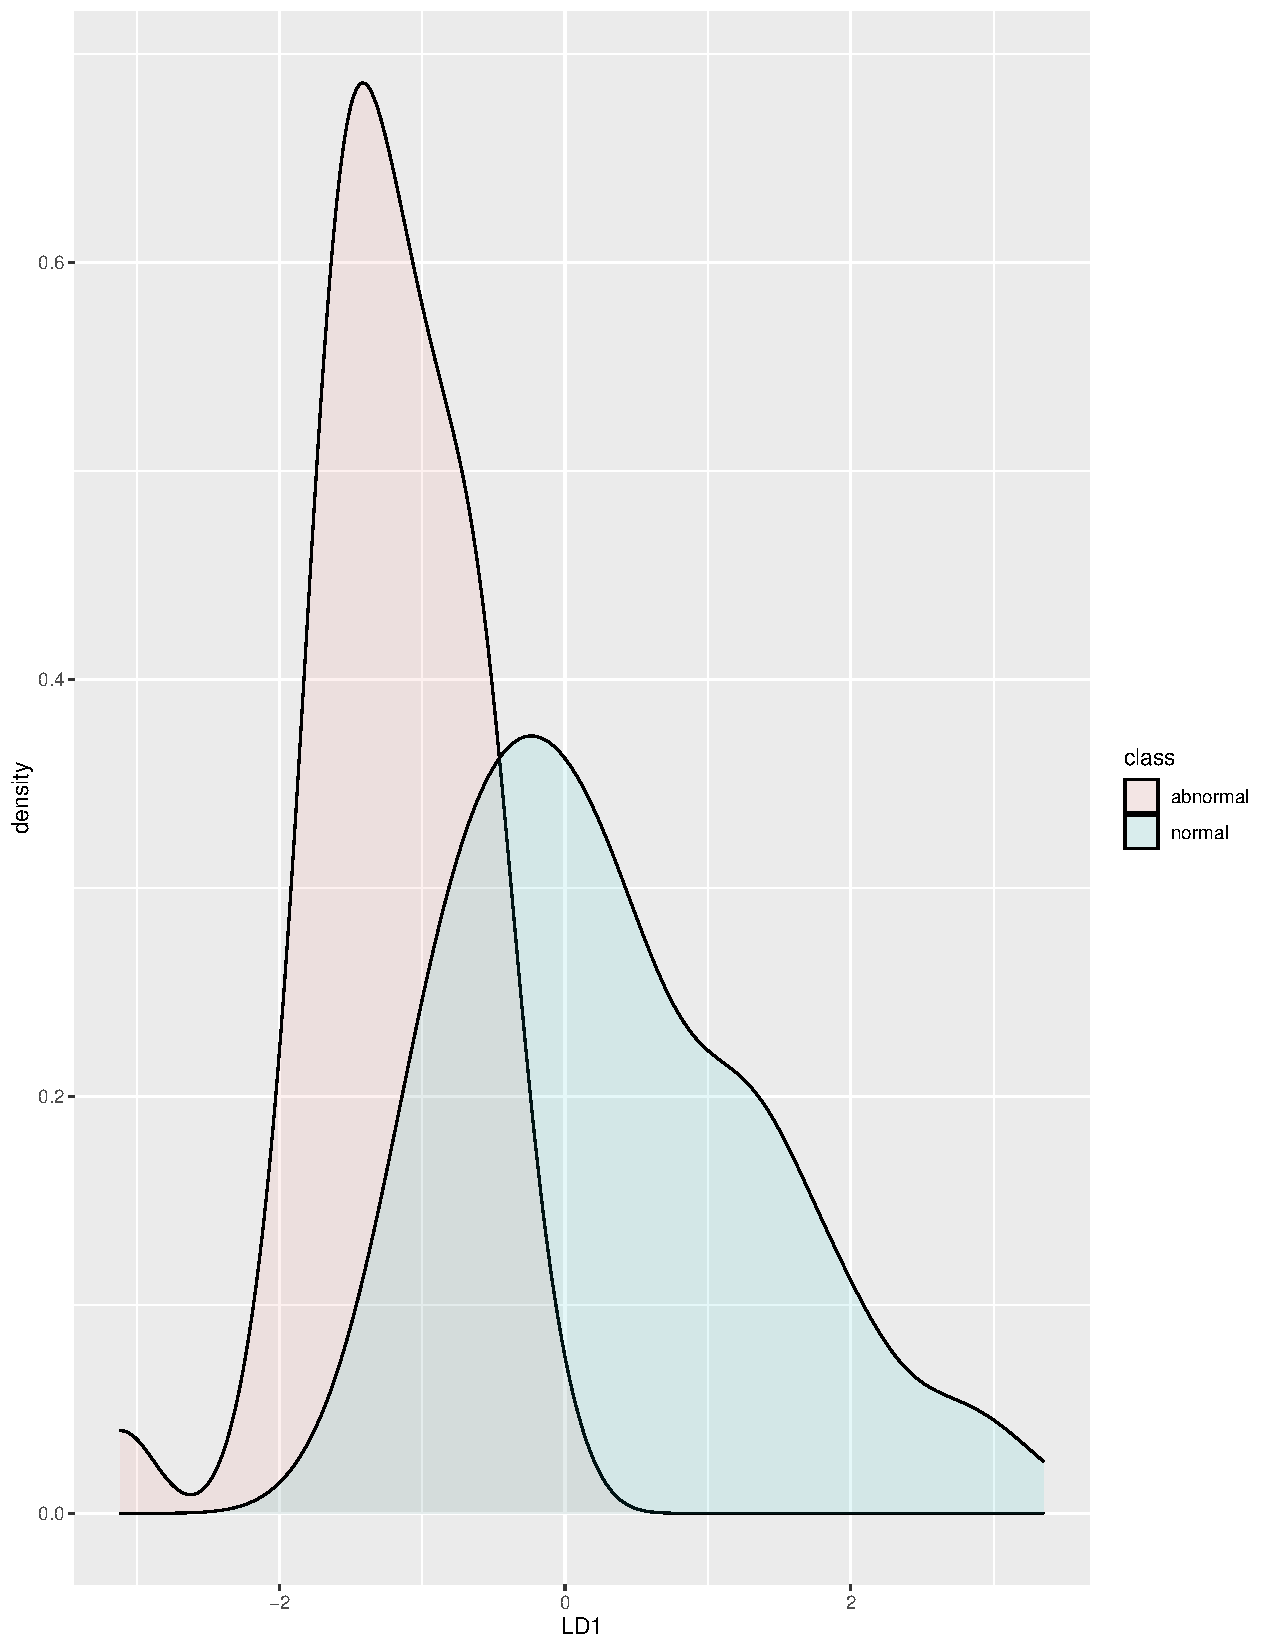
\includegraphics[scale=0.5]{density.pdf}
\caption{Funkcje gęstości wektora zmiennych dyskryminujących dla obu klas przedstawione na jednym wykresie. Widzimy, że klasy nie są jednoznacznie separowalne.}
\end{figure}

Po zbudowaniu klasyfikatora przeszliśmy do jego oceny. Na bazie obserwacji niewykorzystanych do budowy klasyfikatora zbadaliśmy zgodność klasyfikatora z rzeczywistymi danymi. 

\begin{lstlisting}[caption={Macierz pomyłek dla danych treningowych}]
          Actual
predicted  abnormal normal
  abnormal       18      3
  normal         24    158
\end{lstlisting}
Dla danych treningowych osiągnięto precyzję 0.8669951.

\begin{lstlisting}[caption={Macierz pomyłek dla danych testowych}]
          Actual
predicted  abnormal normal
  abnormal        5      3
  normal          8     46
\end{lstlisting}
Dla danych testowych osiągnięto precyzję 0.8225806.



\newpage
\section{Podsumowanie}

\end{document}
